\chapter{Evaluation}

\label{Evaluation} % For referencing the chapter elsewhere, use \ref{Chapter1}


\section{The APK Representation}
\label{sec:apkrepresentation}

\begin{marginfigure}[3\baselineskip] % move figure up by 1 line -5\baselineskip
    \center
    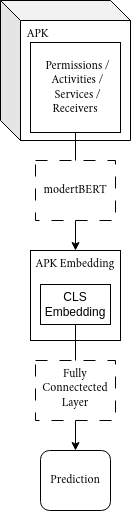
\includegraphics[width=0.6\marginparwidth]{4_Evaluation/permission_transformer_schema.png}
    \caption{\label{fig:permission_transformer_schema}
    Distribution of malware and goodware samples across datasets shown as pie charts.
    The datasets analyzed are are ordered by size from largest to smallest.
    The number of APKs contained in the Dataset are shown in brackets}
\end{marginfigure}

A key aspect of designing an embedding based mobile malware detection system is 
how the APK is represented. Since most embedding models, including all considered BERT models, 
cannot process APKs as a whole, specific features such as permissions, API calls, 
or manifest attributes must be selected and represented in a tokenizable format. 
These features should be structured consistently to ensure comparability across different APKs.

To structure these features, concatenating them with designated tokenizer vocabulary entries 
as separators is beneficial. 
In this work, a varying number of \# characters were used as separators, 
with different separators applied to distinguish between various types of separations 
(e.g., separating feature categories versus separating elements within a feature list).

To show how varying APK representations change the performance of a malware detection 
architecture, an experiment was done with a relatively simple stack 
\ref{fig:permission_transformer_schema}. 
To best see how the representation has an effect, 
the other two variables of the stack were kept static. 
For simplicity and efficiency, the selected embedder was ModernBERT \cite{modernbert}. 
Since ModernBERT has a context window of up to 8000 tokens, 
it was possible to process each APK in one iteration, 
ensuring that the entire representation was captured in a single pass. 
This approach improves efficiency by reducing computational overhead and helps preserve 
relationships within the APKs extracted features. 
The embedding size was set to 768, as recommended by the original ModernBERT authors. 
After applying the Embedding, each input token along a blank CLS token is represented
by 768 floating points.
After each APK was embedded, a simple fully connected layer with dropout was 
trained for 5 epochs on the timebased 
split subset of the dataset, as described in the previous chapter. 
To simplify processing, the decision head was not trained on the full 
embedding but rather only on the CLS token embedding. Each APK was therefore 
represented by 768 floating-point values, ensuring a compact yet 
informative representation for classification.
During training, only the weights of the last fully connected layer were updated, 
while the weights of the ModernBERT embedder were frozen.
The fully connected layer was chosen for its simplicity and effectiveness in 
classification tasks, while the dropout mechanism was included to help prevent overfitting 
and improve generalization. With this stack, 
multiple different APK representations could be chosen. 
However, the representation was limited to 8000 tokens so that it could be 
processed by ModernBERT in a single pass. 
The representations that were chosen were all extracted from the manifest.xml file, 
as it contains important metadata about an application's permissions, activities, services, 
and broadcast receivers, which are often indicative of its behavior and potential security risks. 
The selected ones were the names of the given permissions of the APK, 
the names of the marked activities, 
and the names of the marked services and receivers. 
Permissions indicate what resources an application can access, 
while activities, services, and receivers help determine its execution behavior. 

\begin{table}[b!]
    \caption{\label{tab:apk_representation_results}%
    Performance of different APK representations using frozen ModernBERT embeddings. Features are extracted from Android manifest.xml (A=Activities, P=Permissions, R=Receivers, S=Services). Results reported on time-based transcend subset split after five epochs.}
    \resizebox{\textwidth}{!}{%
    \begin{tabular}{@{}lcccc@{}}
    \toprule
    \textbf{Representation} & \textbf{Accuracy} & \textbf{Precision} & \textbf{Recall} & \textbf{F1} \\ 
    \cmidrule(r){1-1} \cmidrule(lr){2-5}
    A + P + R + S & 74.45\% & 76.30\% & 70.58\% & 73.33\% \\
    A + P + S      & 74.67\% & 76.39\% & 71.09\% & 73.64\% \\
    A + P          & 74.47\% & 74.10\% & 74.89\% & 74.49\% \\
    R + S          & 65.12\% & 74.12\% & 45.97\% & 56.75\% \\
    A              & 70.64\% & 70.88\% & 69.62\% & 70.24\% \\
    P              & 66.51\% & 63.48\% & 77.01\% & 69.60\% \\
    S              & 65.12\% & 69.28\% & 53.77\% & 60.55\% \\
    R              & 50.23\% & 0.00\%  & 0.00\%  & 0.00\%  \\
    \bottomrule
    \end{tabular}%
    }
\end{table}

The performance results in Table \ref{tab:apk_representation_results} 
illustrate how the represention of an APK impacts malware detection. 
The combination of activities, permissions, receivers, and services (A + P + R + S) 
achieved an F1 score of 73.33\%, indicating that a comprehensive manifest representation 
is beneficial. However, removing receivers (A + P + S) 
slightly improved performance to 73.64\%, suggesting that including receivers 
introduces noise that can degrade overall performance.

A subset with only activities and permissions (A + P) produced the highest F1 
score of 74.49\%, confirming that these two features capture essential malicious behaviors 
effectively. Permissions alone (P) showed high recall (77.01\%) 
but not so high precision (63.48\%), 
reflecting the broad use of permissions in both benign and malicious applications. 
Activities (A) offered a balanced performance with an F1 score of 70.24\%, 
indicating  importance in malware detection.

Receivers (R) significantly worsened performance when included, 
resulting in an F1 score of 0.00\% when used alone, and lowering overall 
performance when combined with other features. 
Services (S) also struggled with an F1 score of 60.55\%, 
indicating that these background components, while relevant, 
lack strong discriminative power in isolation. 
Permissions and activities show the most potential as features for static malware detection, 
with the removal of receivers improving overall system robustness.

Comparing the results of this experiment with just permissions as Feature representation with 
the previous results of doing malware detection with a decision tree based on solely 
the permissions (table: \ref{tab:decisiontreepermissions}) shows how promising this architecture is, 
as it shows much better results.
This might be partly due to the analysis of custom permission naming.


\section{The Transformer Encoder}

\label{sec:tran_enc}

\begin{table}[b!]
    \caption{\label{tab:apk_representation_results_unfrozen}%
    Performance of different APK representations using \emph{unfrozen} ModernBERT embeddings. Features are extracted from the Android manifest.xml (A=Activities, P=Permissions, R=Receivers, S=Services). The encoder was also trained through backpropagation in this experiment.}
    \resizebox{\textwidth}{!}{%
    \begin{tabular}{@{}lcccc@{}}
    \toprule
    \textbf{Representation} & \textbf{Accuracy} & \textbf{Precision} & \textbf{Recall} & \textbf{F1} \\ 
    \cmidrule(r){1-1} \cmidrule(lr){2-5}
    A + P + R + S & 83.95\% & 88.67\% & 77.67\% & 82.81\% \\
    A + P + S     & 84.32\% & 85.14\% & 82.99\% & 84.05\% \\
    A + P         & 85.66\% & 87.88\% & 82.58\% & 85.15\% \\
    R + S         & 71.04\% & 87.89\% & 48.51\% & 62.51\% \\
    A             & 80.29\% & 90.22\% & 67.75\% & 77.39\% \\
    P             & 74.97\% & 72.20\% & 80.86\% & 76.28\% \\
    S             & 72.23\% & 88.46\% & 50.84\% & 64.57\% \\
    R             & 50.23\% & 0.00\%  & 0.00\%  & 0.00\%  \\
    \bottomrule
    \end{tabular}%
    }
\end{table}

The second variable of the analyzed Architecture for 
APK classification is the Transformer Encoder 
(Figure \ref{fig:bertbased_malwaredetection_schema}).
Possible Transformer Encoders to use in this approach include: 
BigBird \cite{bigbird}, Longformer \cite{longformer}, 
Performer \cite{performer}, Linformer \cite{linformer},
Reformer \cite{reformer}, FNet \cite{fnet}, 
Nyströformer \cite{nystromformer} or DexBert \cite{dexbert}.
Before any of the listed encoders can encode any language based representation
of the APK, the input first have to be tokenized.
For the tokenization process a vocabulary is needed that maps different tokens
to an integer value. The vocabulary is learned during the training of an encoder model 
and is therefore model specific. In this work it improved the efficiency of 
the pipelines (e.g. Figure \ref{fig:permission_transformer_schema}) 
to first tokenize all of the APK representations before encoding them, 
in order not to create queues of mixed GPU \& CPU usages.

Once tokenized, the general Idea for the Encoder is to reduce the volume of the chosen
APK Representation to a more manageble Level while still maintaining all 
the relevant information that is needed for a classification.
Therefore, models with a large context window are especially suitable.
ModernBERT \cite{modernbert} with its context window of up to 8000 tokens
makes it an especially suitable candidate.
The output of the Encoder is an embedding of the APK representation.
The volume of the embedding is a hyperparameter of the Encoder.
For ModernBERT the default size of the embedding is 768.

The first experiment of this thesis that focuses on the Encoder with regards
to overall model performance bases on the same stack as the previous experiment
(Figure \ref{fig:permission_transformer_schema}).
While the setup stayed mostly the same the only change was to unfreeze the 
encoder models parameters during training. This led ModernBERT to 
also improve its embeddings during training. The results of this is shown in 
table \ref{tab:apk_representation_results_unfrozen}. When comparing these 
results with the results of the previous experiment, where the same 
encoder model was frozen \ref{tab:apk_representation_results}, it becomes 
clear that the performance of the classification increases in nearly every instance.
For the receivers as representation the resulting F1 score stayed 0\% which shows
that without a proper representation a better encoder can not outbalance this.
Other than this instance the performance increased for all representations
for up to more than 10\% points of the F1 score, with stronger increases for
more complex and combined representations. The F1 score of 85.15\% for the 
activities and representations representation shows how well this very simple
and also efficient approach works.

\begin{margintable}[-5\baselineskip]
    \caption{\label{tab:full_transcendence_permissions_a_p} Performance of Activities (A) and Permissions (P) as representations using the full transcending dataset and otherwise the same setup as for table \ref{tab:apk_representation_results_unfrozen}}
    \footnotesize
    \begin{tabular*}{\linewidth}{@{\extracolsep{\fill}} cccc@{}}
        \toprule
        \textbf{Acc.} & \textbf{Prec.} & \textbf{Rec.} & \textbf{F1} \\
        \midrule
        92.57\% & 67.97\% & 67.52\% & 67.74\% \\
        \bottomrule
    \end{tabular*}
\end{margintable}

\begin{margintable}[5\baselineskip]
    \caption{\label{tab:full_transcendence_permissions_a_p_s} Performance of Activities (A), Permissions (P) and Services (S) as representations using the full transcending dataset and otherwise the same setup as for table \ref{tab:apk_representation_results_unfrozen}}
    \footnotesize
    \begin{tabular*}{\linewidth}{@{\extracolsep{\fill}} cccc@{}}
        \toprule
        \textbf{Acc.} & \textbf{Prec.} & \textbf{Rec.} & \textbf{F1} \\
        \midrule
        92.33\% & 67.07\% & 65.98\% & 66.52\% \\
        \bottomrule
    \end{tabular*}
\end{margintable}


Since the performance of that very basic algorithm, that only embeds most basic 
features of the APK, were that promising, another experiment was conducted 
testing the approach on the full Transcend dataset. 
Since they showed the best results, both the A+P and the 
A+P+S representations were selected for this.
The reason not all algorithms were evaluated on the full dataset was of 
computational and time constraints.
Tables \ref{tab:full_transcendence_permissions_a_p} and 
\ref{tab:full_transcendence_permissions_a_p_s} show the metrics achieved on the 
full dataset.
What can be observed is that while the accuracy increases from ~85\% to 
~92\% the precision, recall and f1 scores drop for around 20 percentage points.
The higher accuracy means that the algorithm is right more often on the predictions
of both malware and goodware samples, however the precision and recall show that relatively 
on this dataset the algorithm had more troubles to detect the malware samples.
These changes in performance metrics can be explained by the different label 
class balance. 
In the subsets that have been used in the other experiments, the malware to goodware 
ratio was 1:1, however in the full Transcend dataset there are 11.6\% malware 
and 88.4\% goodware samples.
These results indicate, that the algorithm performance for malware detection decreases 
in settings where labels are unevenly distributed.
This highlights the significance of dataset size in training 
transformer based models for Android malware detection. 

When comparing these results with those in Table \ref{tab:apk_representation_results_unfrozen}, 
we see that using the full dataset leads to a decrease in performance. 
However, the conclusion from the previous experiment remains valid: 
the A+P representation still outperforms the A+P+S representation.
While the results are not directly comparable to other algorithms benchmarked on the 
Transcending dataset, the implication of the experiments are still valuable.

Another Experiment that was conducted in order to evaluate the 
Transformer Encoder in the malware detection architecture is to switch
the base model of the encoder.
For this, APKs were represented by its permissions and activities
and the same transcendence subset was used as in the previous experiments 
(table \ref{tab:apk_representation_results} and \ref{tab:apk_representation_results_unfrozen}).
In this experiment, with the same general setup, three different Encoder basemodels were compared.
In the experiment the encoder model was also trained along the decision head.
The models that were considered were ModernBERT \cite{modernbert}, 
BigBird \cite{bigbird} and Longformer \cite{longformer}. 

When using the same approach as before, where the embedding of the CLS token is used
as the input for the decision head, the performance of the models is as shown in 
table \ref{tab:encoder_model_comparison_cls}. The results for both BigBird and 
Longformer are equally unsatisfactory even though they differ in F1 score.
What happens for both models is that the predictions are either positive or negative for all samples considered. 
Since the metrics are calculated for the malware class only, the recall is either 0\%
or 100\% depending on whether goodware or malware is predicted.

The results for BigBird and Longformer might be that bad, since they use sparse attention
rather fully attention as ModernBERT does.
However, both models claim to use full attentiton for the CLS token.
To verify the general setup, another experiment was done where instead of 
using the embedding of the CLS token
as input for the decision head, the average of all embedded 
tokens was computed along each of their features.
This resulted in better results for both BigBird and Longformer 
while decreasing the performance of
ModernBERT as seen by table \ref{tab:encoder_model_comparison_average}.

During execution, it became obvious that the runtime of BigBird and Longformer were
around 12x slower than ModernBERT even though they only use sparse attention, 
which again makes ModernBERT look superior.
However, it is to be found out if the same models are superior for all kinds of
APK representations. For example DexBERT is trained specifically on Smali code
and is therefore likely to perform better on this as APK representation.

\begin{table}[b] 
    \caption{\label{tab:encoder_model_comparison_cls}%
    Performance comparison of different encoder models for generating embeddings. The APK representation is fixed to Activities (A) and Permissions (P). The encoder was trained through backpropagation in this experiment. The transcenden subset was used as dataset. The embedding of the CLS token was used as APK embedding.}    
    \resizebox{\textwidth}{!}{%
    \begin{tabular}{@{}lcccc@{}}
    \toprule
    \textbf{Model} & \textbf{Accuracy} & \textbf{Precision} & \textbf{Recall} & \textbf{F1} \\ 
    \cmidrule(r){1-1} \cmidrule(lr){2-5}
    ModernBERT & 85.66\% & 87.88\% & 82.58\% & 85.15\% \\
    BigBird    & 49.77\% & 49.77\% & 100.00\% & 66.46\% \\
    Longformer & 50.23\% & 0.00\% & 0.00\% & 0.00\% \\
    \bottomrule
    \end{tabular}%
    }
\end{table}

In addition to the effectiveness also the size and applicability of 
the vocabulary has to be considered. As the vocabulary is the dictionary that
is used when tokenizing the input (the APK representation), the vocabulary 
together with the context window of the model define how much volume the
input is allowed to have. ModernBERT for example has a context window of
8192 while having a vocabulary size of 50368, in comparison: BigBird has 
a context window of 4096 and a vocabulary size of 50358 and Longformer has
a context window of 4096 and a vocabulary size of 30522. This as well makes 
ModernBERT look superior to the alternative models. It is to be considered through
how well the vocabulary fits the input data, as the efficiency is worse for 
words that have to be broken down into multiple smaller tokens instead of being
represented by just one.
Overall ModernBERT seems to be superior to both BigBird and Longformer when used as encoder in 
the malware detection pipeline.


\section{The Decision Head}

\begin{marginfigure}[3\baselineskip] % move figure up by 1 line -5\baselineskip
    \center
    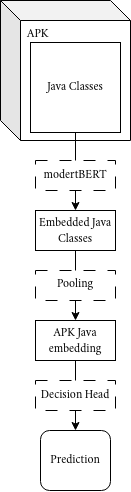
\includegraphics[width=0.6\marginparwidth]{4_Evaluation/java_transformer_schema.png}
    \caption{\label{fig:java_transformer_schema}
    Distribution of malware and goodware samples across datasets shown as pie charts.
    The datasets analyzed are ordered by size from largest to smallest.
    The number of APKs contained in the Dataset are shown in brackets}
\end{marginfigure}


The last of the three variables of the proposed architecture 
\ref{fig:bertbased_malwaredetection_schema}
is the decision head. 
In the experiments so far the decision head was a simple fully connected layer,
that was trained to predict the label from the embedding of the APK representation.
This has proven to be quite effective, however the applicability of this particular 
decision head is limited.
Whenever the tokenized APK representation exceeds the context window of the embedding 
model, the general architecture becomes more complicated.
If the representation cannot be summarized before the embedding, the only solution 
that still bases on a transformer embedding is to break down the representation into 
smaller chunks and to embed these chunks iteratively.
This then leads to one APK not being represented by a single 
embedding but rather by multiple ones.
Especially if the number of chunks the representation has to be broken down into, 
varies in between APKs, it can be difficult to train a common decision head as the 
input of it is of high and potentially varying size.

This issue can be overcome by pooling the embeddings into a smaller and fixed sized
state.
If the representation is of varying size the number of potential pooling mechanisms decreases,
but there are still some possibilities.
One really simple pooling would be to compute the min, max and/or mean of the embeddings.
As the embeddings all have the same size, these statistical measures can just be computed
over each feature of it.
Another approach would be to select one of the representations by random.

In order to evaluate what kinds of decision heads perform better or worse on 
the task of embedding classification another experiment was conducted.
While it still shows the general structure of the proposed architecture 
\ref{fig:bertbased_malwaredetection_schema}, it differs quite a bit from the 
previous setup shown in Figure \ref{fig:permission_transformer_schema}.
Figure \ref{fig:java_transformer_schema} shows how this new experiment is set up.
As the representation of each APK, the java code that can be decompiled from the
classes.dex file is used. This java code is then structured by the corresponding
classes. This representation is quite extensive as it consists of 1866
classes on average on the full transcending dataset \ref{fig:java_class_boxplots}.
This brings the base architecture \ref{fig:permission_transformer_schema} to
the following problem: In most cases the APK representation exceeds the context
window of the ModernBERT model that is used to calculate the embeddings.
As discussed before, the Representation has therefore to be broken down into chunks.
For Chunks the java classes were used. While this is an easy way to break down the code,
even single java classes sometimes exceed the 8000 tokens that defines the 
ModernBERT context window. If this occurred during the experiment, the java class was
processed in multiple iterations via a sliding window approach with a stride of 6000.
Then only for those cases, the average of each CLS token, that was generated with the
sliding window, was used for the APK representation. 
Like this one CLS token for each java class was computed.

\begin{margintable}[-5\baselineskip]
    \caption{\label{tab:matching_java_classes_transcend} Number of total java classes and classes that are mentioned by the manifest.xml file of the Transcending dataset. Also the number of classes that match by the classname is given}
    \footnotesize
    \begin{tabular*}{\linewidth}{@{\extracolsep{\fill}} lcr@{}}
        \toprule
        \textbf{Feature} & \textbf{Mean} & \textbf{Sum} \\
        \midrule
        Java Classes & 1866 & 483102763 \\
        Manifest Classes & 20 & 5277764 \\
        Matching Classes & 14 & 3791740 \\
        \bottomrule
    \end{tabular*}
\end{margintable}


One approach, that was tried to reduce the amount of java classes that had to be embedded, 
was to only process those java classes that are either declared as activities, permissions, services or receivers in the
Manifest.xml file. This approach was not feasible due to some obfuscation technique that
changed the naming of the java classes in the manifest file. Deeper analysis showed
that only 72\% (see table \ref{tab:matching_java_classes_transcend}) of java classes in the transcending dataset have a constant naming
between classes.dex and manifest.xml file. For the DexRay dataset it even were only
12\% (see table \ref{tab:matching_java_classes_dexray}). So all the java classes of the APK were considered.

\begin{margintable}[-5\baselineskip]
    \caption{\label{tab:matching_java_classes_dexray} Number of total java classes and classes that are mentioned by the manifest.xml file of the DexRay dataset. Also the number of classes that match by the classname is given}
    \footnotesize
    \begin{tabular*}{\linewidth}{@{\extracolsep{\fill}} lcr@{}}
        \toprule
        \textbf{Feature} & \textbf{Mean} & \textbf{Sum} \\
        \midrule
        Java Classes & 1394 & 220838917 \\
        Manifest Classes & 58 & 9247905 \\
        Matching Classes & 7 & 1126716 \\
        \bottomrule
    \end{tabular*}
\end{margintable}


As stated before this led to a variable size embedding that
has to be classified.
The experiment that is conducted to evaluate the decision heads is based on 
the approach of \cite{detectbert}. Therefore, the detectBERT model is used as 
Decision head as well as three other simple approaches and their performance 
is compared.
The other approaches are: 
Average - here the mean of all the Java Class based
CLS token embeddings is computed and then processed by a fully connected layer.
The mean is computed for each of the 768 features the Embedding has, so that the
resulting mean embedding has 768 features as well;
Addition - the same as with Average but instead of the mean, the sum is used to
derive a single embedding that represents the APK;
Random - here one java class is selected randomly and its CLS Embedding is used to 
represent the APK for the classification task.

Table \ref{tab:decision_head_comparison} shows the results of the conducted experiment.
The performance is evaluated after training the decision head for 20 epochs on 
the same transcendence subset that is used in previous experiments. This subset 
is split into train and test sets sequentially to account for concept drift.

\begin{table}[b]
    \centering
    \caption{\label{tab:decision_head_comparison}Performance comparison of different decision heads on the Transcend dataset with a time-based split.}
    \resizebox{\textwidth}{!}{%
    \begin{tabular}{@{}lcccc@{}}
    \toprule
    \textbf{Decision Head} & \textbf{Accuracy} & \textbf{Precision} & \textbf{Recall} & \textbf{F1} \\ 
    \cmidrule(r){1-1} \cmidrule(lr){2-5}
    Average    & 83.00\% & 84.85\% & 80.35\% & 82.54\% \\
    Addition   & 59.15\% & 55.52\% & 92.00\% & 69.25\% \\
    DetectBERT & 74.28\% & 90.70\% & 54.10\% & 67.77\% \\
    Random     & 66.18\% & 67.13\% & 63.40\% & 65.21\% \\
    \bottomrule
    \end{tabular}%
    }
\end{table}

The average aggregation of CLS tokens achieved the best overall results, 
demonstrating high accuracy (83.00\%), precision (84.85\%), recall (80.35\%), 
and F1 score (82.54\%). This indicates balanced performance, 
effectively minimizing both false positives and false negatives.
The DetectBERT decision head showed moderate accuracy (74.28\%) 
and exceptionally high precision (90.7\%), but considerably lower recall (54.10\%). 
This indicates that while it rarely produces false positives, 
it frequently overlooks actual positives. 
The "Addition" decision head shows the highest recall (92.00\%) but low precision 
(55.52\%) and low accuracy (59.15\%). 
This approach is beneficial in applications where missing true positives is highly 
undesirable, even if it leads to many false positives. For example this could be useful 
for the task of identifying high risk APKs.
Lastly, the "Random" decision head serves as a baseline, 
performing modestly across all metrics (Accuracy: 66.18\%, Precision: 67.13\%, 
Recall: 63.40\%, F1: 65.21\%), 
highlighting the relative improvements of the other methods.
In terms of F1 score, both the Addition and DetectBERT approach perform only slightly better 
than the Random approach.
Overall the ranking of the four decision heads that are used is quite different from the 
performances reported on the smali embeddings by \cite{detectbert}, which does seem to 
overestimate the performance of DetectBERT.

In the chapter \ref{sec:detectbert} we evaluated the DetectBERT decision head on the same 
dataset with the same split but on smali based embeddings calculated by dexBERT rather 
than java based embeddings calculate by ModernBERT. 
The DetectBERT head achieved improved performance on these embeddings, 
obtaining an accuracy of 80.13\%, precision of 80.91\%, recall of 78.88\%, and an F1-score of 79.88\% 
as shown in table \ref{tab:detectbert-results}.
Compared to the Java based embeddings, this indicates that DetectBERT performs significantly better 
with smali based embeddings, especially regarding recall, 
indicating that the choice of the decision head does depend on the type of embedding that is used.

The decreased effectiveness of the DetectBERT decision when comparing our results with the results 
reported by DetectBERT (97\% F1 score; table \ref{tab:detectbert_performance_original}) might be explained 
by the dataset that has been used. While the transcend subset that we used seems to be an easier benchmark 
than the full trancend dataset, it was balanced on the amount of smali and java classes between labels.
If DetectBERT works similarly to the aggregation head, in a sense that the amount of classes 
that are embedded have a direct impact on the prediction derived, this drop can be explained.
We showed in chapter \ref{sec:datasets} that the dexRay dataset, that was used for the experiments that 
led to the 97\% F1 score, is highly imbalanced in terms of smali classes between labels as visualized by the 
boxplot in figure \ref{fig:smali_class_boxplots}.